\documentclass[tikz,border=2mm, convert]{standalone}

\begin{document}
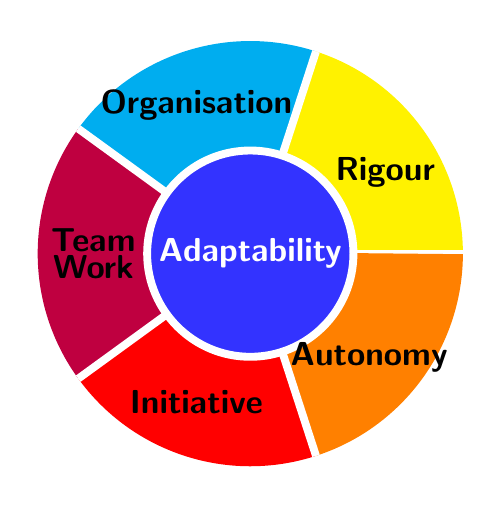
\begin{tikzpicture}[font=\sffamily\bfseries\large, 
     text=black, 
     border/.style={line width=14mm}]
\foreach \angle/\col [remember=\angle as \last (initially 0)] in 
    {72/yellow, 144/cyan, 216/purple, 288/red, 360/orange}{
        \draw[\col, border] (\last:2cm) 
             arc[start angle=\last, end angle=\angle, radius=2cm];
        \draw[white, line width=1mm] (\last:1.3)--++(\last:1.4);
}
\node[line width=1mm, draw, circle, minimum width=2.5cm, white, fill=blue!80] {Adaptability};
\node at (31:2cm) {Rigour};
\node at (110:2cm) {Organisation};
\node at (175:2cm) {Team};
\node at (185:2cm) {Work};
\node at (250:2cm) {Initiative};
\node at (319:2cm) {Autonomy};
\end{tikzpicture}
\end{document}

